\chapter{System Overview}

The goal of the system is to classify panorama images into predefined classes.  
For this, a CLIP-like network is used at the edge.  
The computing platform consists of a Raspberry Pi 5 with the hardware accelerator extension.  
The hardware accelerator is the Hailo-8L entry-level accelerator (\cref{fig:overview:aikit}).  

The system used and developed in this work can be divided into two parts.  
One part involves compiling a neural network on a PC,  
while the other part focuses on running the inference of the compiled network on the Raspberry Pi.

\begin{figure}[h]
    \centering
    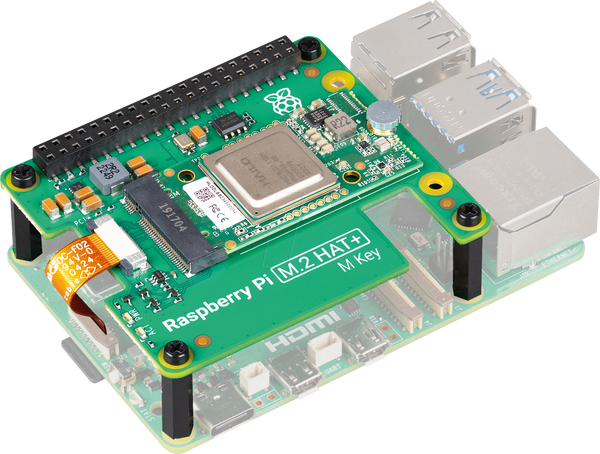
\includegraphics[width=0.5\textwidth]{Images/SystemOverview/ai-kit.png}
    \caption{Picture of the hardware accelerator mounted on a Raspberry Pi 5\cite{bildAiKit}}
    \label{fig:overview:aikit}
\end{figure}



\section{Compilation of a Network}

\begin{figure}
    \centering
    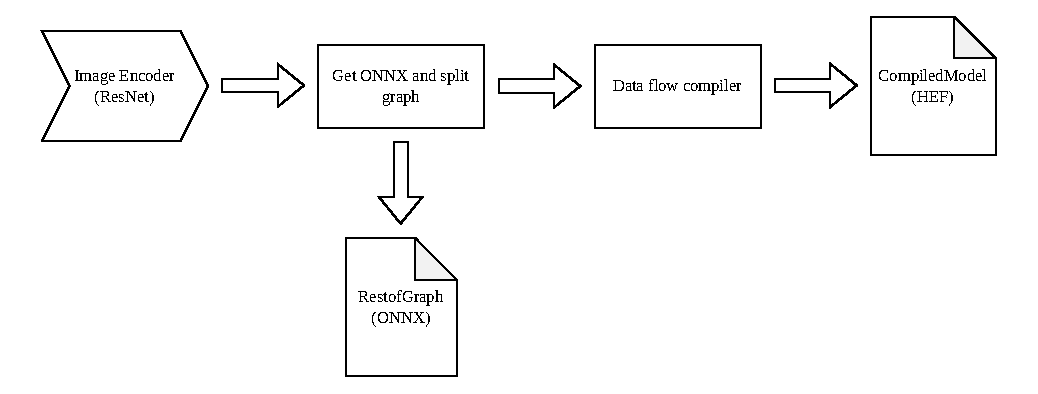
\includegraphics[width=0.8\textwidth]{Images/SystemOverview/DFCFlow.pdf}
    \caption{Visualization of the compilation workflow}
    \label{fig:overview:dfcflow}
\end{figure}

First, the image encoder, either from \acrshort{clip} or TinyCLIP, must be acquired.  
This encoder is then exported as an ONNX graph.  
Any part of the graph that cannot be compiled is removed and saved for later use.  
The edited graph is then compiled.  
During compilation, the network undergoes quantization and simplification.  
This reduces the memory and processing power required to run the network.  

The network must be compiled into a format that can be executed on the hardware accelerator.  
In this work, the compilation is performed using the \Acrlong{dfc} (see \cref{section:dfc}) from Hailo.  
The result is a \acrshort{hef} file, which can be executed on Hailo hardware.
All the files then need to be downloaded to the Raspberry Pi.
\begin{figure}[h!]
    \centering
    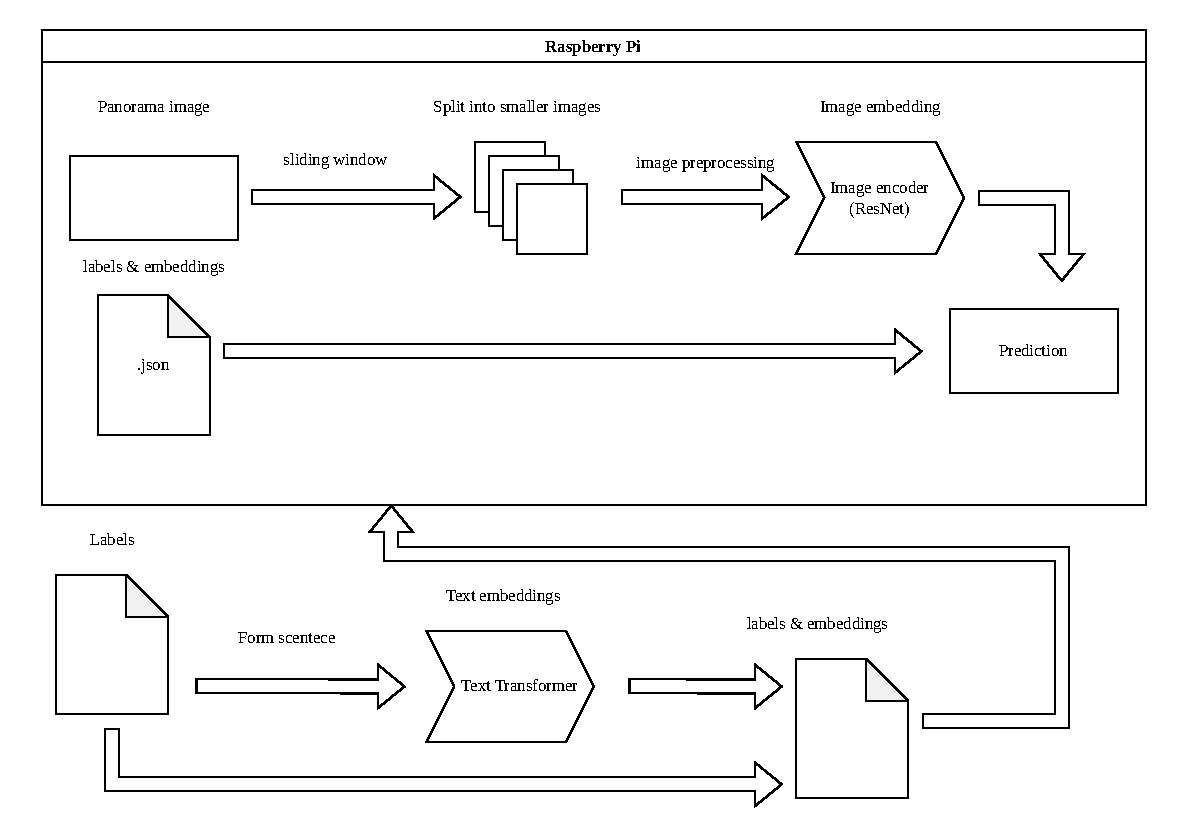
\includegraphics[width=\textwidth]{Images/SystemOverview/Overview.drawio.pdf}
    \caption{System workflow}
    \label{fig:overview:overview}
\end{figure}

\section{Inference on Raspberry Pi}

To use a network on a hardware accelerator, specific software must be employed.  
Due to current limitations of the \acrshort{dfc}, self-attention layers were unable to compile.  
As a result, the text encoder of CLIP must be executed in advance on a PC.  
The resulting text embeddings are then loaded onto the Raspberry Pi in the form of a JSON file.  
The text embeddings consist of the expressions from \cref{tab:dataset:subclasses} subclasses.  
These expressions are wrapped into 5 sentences to improve accuracy.  

The limitation that self-attention layers were unable to compile also prevents the compilation of Transformers.  
Therefore, ResNets were used as the image encoders.  
However, a challenge arose with ResNets, as the last layer is also a self-attention layer.  
To enable the network to compile, the last part of the ResNet was removed and processed later as part of postprocessing.  

The panorama images are divided into 5 separate patches, each classified individually.  
To obtain the final prediction, a majority vote is taken across the 5 image patches.

\begin{figure}[!h]
    \centering
    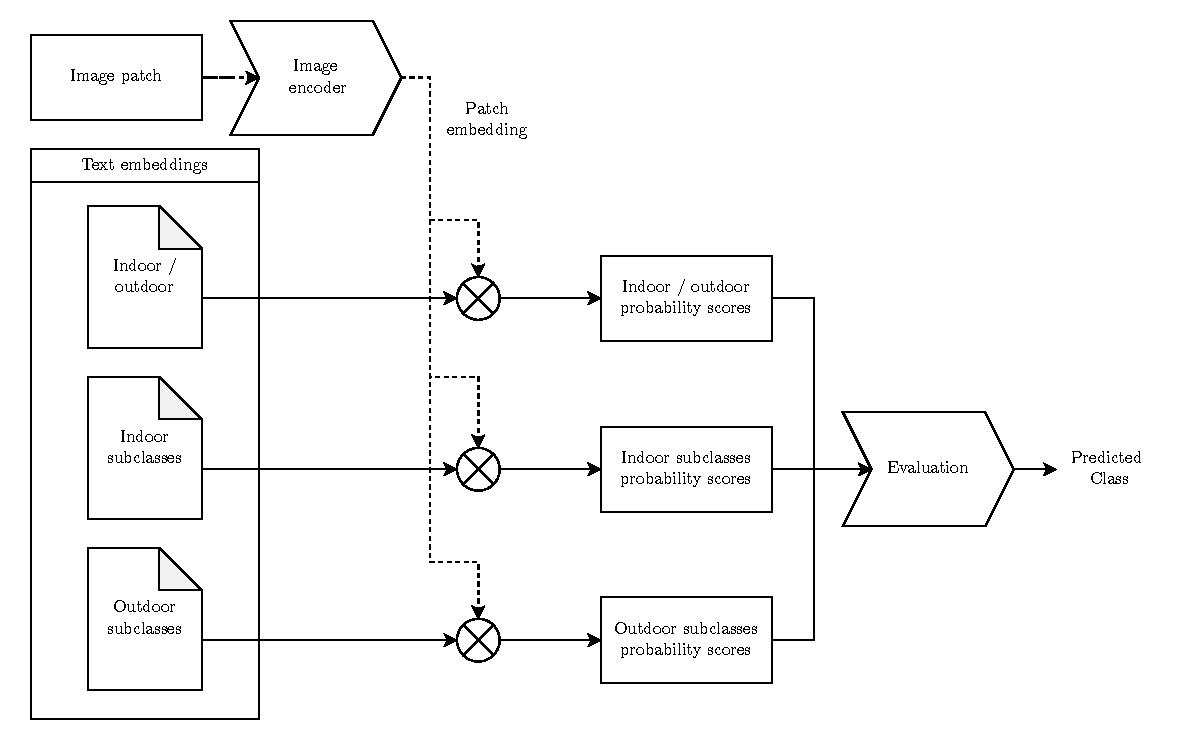
\includegraphics[width=\textwidth]{Images/SystemOverview/Evalution.pdf}
    \caption{This figure shows how a prediction is obtained on the Raspberry Pi}
    \label{fig:overview:evaluation}
\end{figure}

Each patch is embedded by the vision encoder.
To get the probability scores, the text embeddings are loaded from the JSON file and multiplied by the patch embedding.
The text embeddings have 3 layers.
Each layer is computed separately.
The first layer contains the text embeddings to classify a patch as indoor or outdoor.
The second layer is filled with text embeddings from the subclasses of \cref{tab:dataset:subclasses} used in indoor classes.
The third and final layer uses the remaining outdoor subclasses from \cref{tab:dataset:subclasses}.
All these scores are calculated and stored.
Then the evaluation begins.
First, the indoor and outdoor probability scores are compared.
The higher score determines which subclasses are used.
To get the final class, the probability scores of a subclass are summed and compared to the other subclasses.
The highest class is the resulting class.
This process can be seen in \cref{fig:overview:evaluation}.

